\documentclass[
]{jss}

%% recommended packages
\usepackage{orcidlink,thumbpdf,lmodern}

\usepackage[utf8]{inputenc}

\author{
Hanne I. Oberman\\Methodology and Statistics\\
Utrecht University \And Johanna Muñoz\\Julius Center for Health Sciences
and Primary Care,\\
University Medical Center Utrecht, Utrecht University,\\
Utrecht, The Netherlands \AND Thomas P. A. Debray\\Julius Center
for Health Sciences and Primary Care,\\
University Medical Center Utrecht, Utrecht University,\\
Utrecht, The Netherlands \And Gerko Vink\\Methodology and Statistics\\
Utrecht University \AND Valentijn M. T. de Jong\\Julius Center for
Health Sciences and Primary Care,\\
University Medical Center Utrecht, Utrecht University,\\
Utrecht, The Netherlands
}
\title{Imputation of Incomplete Multilevel Data with \pkg{mice}}

\Plainauthor{Hanne I. Oberman, Johanna Muñoz, Thomas P. A. Debray, Gerko
Vink, Valentijn M. T. de Jong}
\Plaintitle{Imputation of Incomplete Multilevel Data with mice}
\Shorttitle{Multilevel \pkg{mice}}


\Abstract{
This tutorial illustrates the imputation of incomplete multilevel data
with the \proglang{R} packackage \pkg{mice}.
}

\Keywords{missing
data, multilevel, clustering, \pkg{mice}, \proglang{R}}
\Plainkeywords{missing data, multilevel, clustering, mice, R}

%% publication information
%% \Volume{50}
%% \Issue{9}
%% \Month{June}
%% \Year{2012}
%% \Submitdate{}
%% \Acceptdate{2012-06-04}

\Address{
    Hanne I. Oberman\\
    Methodology and Statistics\\
Utrecht University\\
    Padualaan 14\\
3584 CH Utrecht\\
  E-mail: \email{h.i.oberman@uu.nl}\\
  URL: \url{https://hanneoberman.github.io/}\\~\\
          }


% tightlist command for lists without linebreak
\providecommand{\tightlist}{%
  \setlength{\itemsep}{0pt}\setlength{\parskip}{0pt}}

% From pandoc table feature
\usepackage{longtable,booktabs,array}
\usepackage{calc} % for calculating minipage widths
% Correct order of tables after \paragraph or \subparagraph
\usepackage{etoolbox}
\makeatletter
\patchcmd\longtable{\par}{\if@noskipsec\mbox{}\fi\par}{}{}
\makeatother
% Allow footnotes in longtable head/foot
\IfFileExists{footnotehyper.sty}{\usepackage{footnotehyper}}{\usepackage{footnote}}
\makesavenoteenv{longtable}


\usepackage{graphicx}
\usepackage{mathtools}
\usepackage{ulem}

\usepackage{amsmath}

\begin{document}



\hypertarget{introduction}{%
\section{Introduction}\label{introduction}}

Many datasets include individuals that are clustered together, for
example in geographic regions, or even different studies. In the
simplest case, individuals (e.g., students) are nested within a single
cluster (e.g., school classes). More complex clustered structures may
occur when there are multiple hierarchical levels (e.g., students in
different schools or patients within hospitals within regions across
countries), or when the clustering is non-nested (e.g., electronic
health record data from diverse settings and populations within large
databases). With clustered data we generally assume that individuals
from the same cluster tend to be more similar than individuals from
other clusters. In statistical terms, this implies that observations
from the same cluster are not independent and may in fact be correlated.
If this correlation is left unaddressed, estimates of \emph{p} values,
confidence intervals even model parameters are prone to bias
\citep{loca01}. Statistical methods for clustered data typically adopt
hierarchical models that explicitly describe the grouping of
observations. These models are also known as `multilevel models',
`hierarchical models', `mixed effect models', `random effect models',
and in the context of time-to-event data as `frailty models'. Table
\ref{tab:clus} provides an overview of some key concepts in multilevel
modeling.

Table 1: Concepts in multilevel methods

\begin{longtable}[]{@{}
  >{\raggedright\arraybackslash}p{(\columnwidth - 2\tabcolsep) * \real{0.2100}}
  >{\raggedright\arraybackslash}p{(\columnwidth - 2\tabcolsep) * \real{0.7900}}@{}}
\toprule()
\begin{minipage}[b]{\linewidth}\raggedright
\textbf{Concept}
\end{minipage} & \begin{minipage}[b]{\linewidth}\raggedright
\textbf{Details}
\end{minipage} \\
\midrule()
\endhead
Sample unit & Units of the population from which measurements are taken
in a sample. \\
Hierarchical levels & Data are grouped into clusters at different
levels. A three-level \\
Fixed effect & Here we assume that the values of an independent variable
are fixed, i.e., \\
& the values observed in the study are representative of all values in
the \\
& in the dependent variable y e.g., blood pressure between treatments A
and B. \\
Random effect & The values of an independent variable are assumed to be
randomly drawn from \\
& admission we might select only certain hospitals that are
representative of \\
& the difference of y between individual hospitals, but rather the
variation of \\
ICC & The variability due to clustering is often measured by means of
the \\
& intraclass coefficient (ICC). The ICC can be seen as the percentage \\
& of variance that can be attributed to the cluster-level, where a
high \\
& ICC would indicate that a lot of variability is due to the cluster \\
& structure. \\
Random effect & Multilevel models typically accommodate for variability
by including \\
& a separate group mean for each cluster. In addition to random \\
& intercepts, multilevel models can also include random coefficients \\
& and heterogeneous residual error variances across clusters {[}see
e.g. \\
& \citet{gelm06}, \citet{hox17} and \citet{jong21}{]}. {[}TODO: add
stratified intercept as concept..{]} \\
\bottomrule()
\end{longtable}

\hypertarget{missingness-in-multilevel-data}{%
\subsection{Missingness in multilevel
data}\label{missingness-in-multilevel-data}}

As with any other dataset, clustered datasets may be impacted by
missingness in much the same way. Several strategies can be used to
handle missing data, including complete case analysis and imputation. We
focus on the latter approach and discuss statistical methods for
replacing the missing data with one or more plausible values. Imputation
separates the missing data problem from the analysis and the completed
data can be analyzed as if it were completely observed. It is generally
recommended to impute the missing values more than once to preserve
uncertainty due to missingness and to allow for valid inferences (c.f.
Rubin 1976).

With incomplete clustered datasets we can distinguish between two types
of missing data: sporadic missingness and systematic missingness
\citep{resc13}. Sporadic missingness arises when variables are missing
for some but not all of the units in a cluster \citep{buur18, jola18}.
For example, it is possible that test results are missing for several
students in one or more classes. When all observations are missing
within one or more clusters, data are said to be systematically missing.

\begin{CodeChunk}
\begin{figure}

{\centering 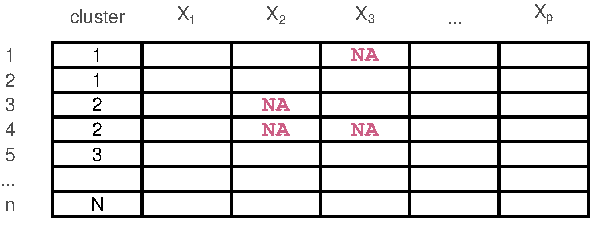
\includegraphics{Imputation_of_Incomplete_Multilevel_Data_files/figure-latex/patterns-1} 

}

\caption[Sporadic missingness in multilevel data]{Sporadic missingness in multilevel data}\label{fig:patterns}
\end{figure}
\end{CodeChunk}

Imputation of missing data requires consideration of the mechanism
behind the missingness. Rubin proposed to distinguish between data that
are missing completely at random (MCAR), data that are missing at random
(MAR) and data that are missing not at random (MNAR; see Table
\ref{tab:miss}). For each of these three missingness generating
mechanisms, different imputation strategies are warranted
(\citet{yuce08} and \citet{hox15}). We here consider the general case
that data are MAR, and expand on certain MNAR situations.

Table 2: Concepts in missing data methods

\begin{longtable}[]{@{}
  >{\raggedright\arraybackslash}p{(\columnwidth - 2\tabcolsep) * \real{0.1739}}
  >{\raggedright\arraybackslash}p{(\columnwidth - 2\tabcolsep) * \real{0.8261}}@{}}
\toprule()
\begin{minipage}[b]{\linewidth}\raggedright
\textbf{Concept}
\end{minipage} & \begin{minipage}[b]{\linewidth}\raggedright
\textbf{Details}
\end{minipage} \\
\midrule()
\endhead
MCAR & Missing Completely At Random, where the probability to be missing
is equal \\
& across all data entries \\
MAR & Missing At Random, where the probability to be missing depends on
observed \\
& information \\
MNAR & Missing Not At Random (MNAR), where the probability to be
missing \\
& depends on unrecorded information, making the missingness
non-ignorable \\
& \citep{rubi76, meng94}. \\
& \\
\bottomrule()
\end{longtable}

\hypertarget{aim-of-this-paper}{%
\subsection{Aim of this paper}\label{aim-of-this-paper}}

This papers serves as a tutorial for imputing incomplete multilevel data
with \pkg{mice} in \proglang{R}. \pkg{mice} has become the de-facto
standard for imputation by chained equations, which iteratively solves
the missingness on a variable-by-variable basis. \pkg{mice} is known to
yield valid inferences under many different missing data circumstances
\citep{buur18}.

We provide practical guidelines and code snippets for different missing
data situations, including non-ignorable mechanisms. For reasons of
brevity, we focus on multilevel imputation by chained equations with
\pkg{mice} exclusively; other imputation methods and packages \citep[see
e.g.][ and \citet{grun18}]{audi18} are outside the scope of this
tutorial. Assumed knowledge includes basic familiarity with the
\pkg{lme4} notation for multilevel models (see Table \ref{tab:mod}).

Table 3: Notation

\begin{longtable}[]{@{}
  >{\raggedright\arraybackslash}p{(\columnwidth - 2\tabcolsep) * \real{0.5495}}
  >{\raggedright\arraybackslash}p{(\columnwidth - 2\tabcolsep) * \real{0.4505}}@{}}
\toprule()
\begin{minipage}[b]{\linewidth}\raggedright
\textbf{Formula \pkg{lme4}}
\end{minipage} & \begin{minipage}[b]{\linewidth}\raggedright
\textbf{Details}
\end{minipage} \\
\midrule()
\endhead
\texttt{y\ \textasciitilde{}\ x1\ +\ (1\ \textbar{}\ g1)} & Fixed
\texttt{x1} predictor with random intercept \\
& varying among \texttt{g1} \\
\texttt{y\textasciitilde{}x1*x2+\ (1\textbar{}\ g1)} & Interactions of
\texttt{x1} and \texttt{x2} only in fixed effect \\
\texttt{y\ \textasciitilde{}\ x1*x2+\ (x2\textbar{}\ g1)} & Interactions
of \texttt{x1} and \texttt{x2} only in fixed effect \\
& with slope of \texttt{x2} randomly varying among \texttt{g1} \\
\texttt{y\ \textasciitilde{}\ x1*x2+\ (x1*x2\textbar{}\ g1)} &
variance-covariance matrix estimated only with \\
& the variance terms of intercept, slope of \texttt{x1}, \\
& slope of \texttt{x2} and interaction \texttt{x1*x2} \\
\texttt{y\ \textasciitilde{}\ x1*x2+\ (x1\ \textbar{}\ g1)+\ (x2\textbar{}\ g1)}
& variance-covariance matrix estimated separately, \\
& i.e, one for intercept and \texttt{x1} and another for \\
& intercept and \texttt{x2} \\
\texttt{y\ \textasciitilde{}\ x1\ +\ (x1\ \textbar{}\ g1)\ or\ 1\ +\ x1\ +\ (1\ +\ x1\ \textbar{}\ g1)}
& Fixed \texttt{x1} with correlated random intercept and \\
& random slope of \texttt{x} \\
\texttt{y\ \textasciitilde{}\ x1\ +\ (x1\ \textbar{}\textbar{}\ g1)\ or\ 1\ +\ x1\ +\ (1\ \textbar{}\ g1)\ +\ (0\ +\ x1\ \textbar{}\ g1)}
& Fixed \texttt{x1} with uncorrelated random intercept \\
& and random slope of \texttt{x1} \\
\texttt{y\ \textasciitilde{}\ (1\ \textbar{}\ g1)\ +\ (1\ \textbar{}\ g2)}
& Random intercept varying among \texttt{g1} and among
\texttt{g2\ \ \ \textbar{}\ \textbar{}}y \textasciitilde{} (1 \\
& \\
\bottomrule()
\end{longtable}

We illustrate imputation of incomplete multilevel data using three case
studies:

\begin{itemize}
\tightlist
\item
  \texttt{popmis} from the \pkg{mice} package \citep[simulated data on
  perceived popularity, \(n = 2,000\) pupils across \(N = 100\) schools
  with data that are MAR,][]{mice};
\item
  \texttt{impact} from the \pkg{metamisc} package \citep[empirical data
  on traumatic brain injuries, \(n = 11,022\) patients across \(N = 15\)
  studies with data that are MAR,][]{metamisc};
\item
  \texttt{obesity} from the \pkg{miceheckman} package {[}simulated data
  on obesity, \(n = 2,111\) patients across \(N = 5\) regions with data
  that are MNAR{]}.
\end{itemize}

For each of these datasets, we discuss the nature of the missingness,
choose one or more imputation models and evaluate the imputed data, but
we will also highlight one specific aspect of the imputation workflow.

This tutorial is dedicated to readers who are unfamiliar with multiple
imputation. More experienced readers can skip the introduction (case
study 1) and directly head to practical applications of multilevel
imputation under MAR conditions (case study 2) or under MNAR conditions
(case study 3).

\hypertarget{setup}{%
\subsection{Setup}\label{setup}}

Install non-CRAN packages if necessary:

\begin{CodeChunk}
\begin{CodeInput}
R> devtools::install_github("amices/ggmice")
R> devtools::install_github("hanneoberman/miceheckman")
\end{CodeInput}
\end{CodeChunk}

Set up the R environment and load the necessary packages:

\begin{CodeChunk}
\begin{CodeInput}
R> set.seed(2022)        # for reproducibility
R> library(mice)         # for imputation
R> library(miceadds)     # for additional imputation routines
R> library(ggmice)       # for incomplete/imputed data visualization
R> library(ggplot2)      # for visualization
R> library(dplyr)        # for data wrangling
R> library(lme4)         # for multilevel modeling
R> library(mitml)        # for multilevel parameter pooling
R> library(miceheckman)  # for imputation cf heckman models
\end{CodeInput}
\end{CodeChunk}

\hypertarget{case-study-i-popularity-data}{%
\section{Case study I: popularity
data}\label{case-study-i-popularity-data}}

In this section we'll go over the different steps involved with imputing
incomplete multilevel data with the R package mice. We consider the
simulated \texttt{popmis} dataset, which included pupils (\(n = 2000\))
clustered within schools (\(N = 100\)). The following variables are of
primary interest:

\begin{itemize}
\tightlist
\item
  \texttt{school}, school identification number (clustering variable);
\item
  \texttt{popular}, pupil popularity (self-rating between 0 and 10;
  unit-level);
\item
  \texttt{sex}, pupil sex (0=boy, 1=girl; unit-level);
\item
  \texttt{texp}, teacher experience (in years; cluster-level).
\end{itemize}

The research objective of the \texttt{popmis} dataset is to predict the
pupils' popularity based on their gender and the experience of the
teacher. The analysis model corresponding to this dataset is multilevel
regression with random intercepts, random slopes and a cross-level
interaction. The outcome variable is \texttt{popular}, which is
predicted from the unit-level variable \texttt{sex} and the
cluster-level variable \texttt{texp}:

\begin{CodeChunk}
\begin{CodeInput}
R> mod <- popular ~ 1 + sex + (1 | school)
\end{CodeInput}
\end{CodeChunk}

The true effect is:

\begin{CodeChunk}


\begin{center}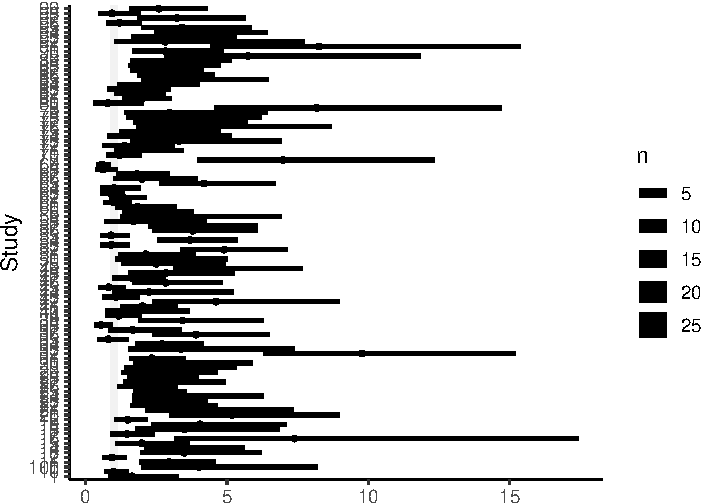
\includegraphics{Imputation_of_Incomplete_Multilevel_Data_files/figure-latex/unnamed-chunk-3-1} \end{center}

\end{CodeChunk}

Load the data into the environment and select the relevant variables:

\begin{CodeChunk}
\begin{CodeInput}
R> popmis <- popmis[, c("school", "popular", "sex")] 
\end{CodeInput}
\end{CodeChunk}

Plot the missing data pattern:

\begin{CodeChunk}
\begin{CodeInput}
R> plot_pattern(popmis, square = TRUE)
\end{CodeInput}
\begin{figure}

{\centering 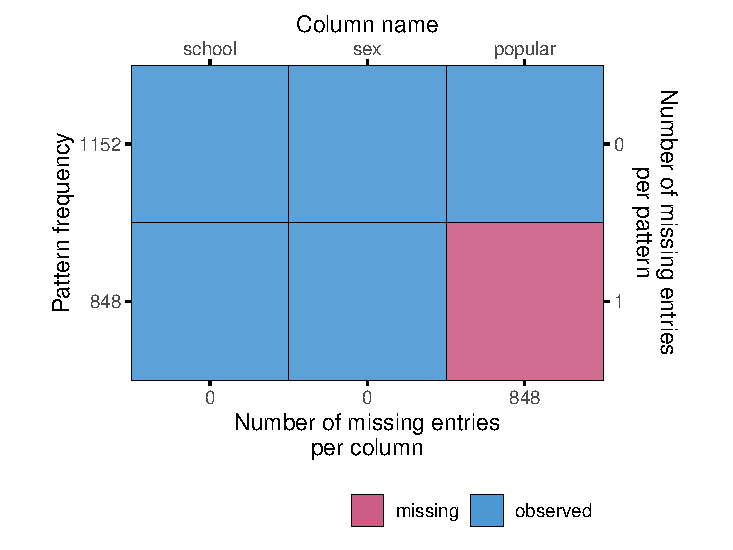
\includegraphics{Imputation_of_Incomplete_Multilevel_Data_files/figure-latex/pop_pat-1} 

}

\caption[Missing data pattern in the popularity data]{Missing data pattern in the popularity data}\label{fig:pop_pat}
\end{figure}
\end{CodeChunk}

The missingness is univariate and sporadic, which is illustrated in the
missing data pattern in Figure \ref{fig:pop_pat}.

To develop the best imputation model for the incomplete variable
\texttt{popular}, we need to know whether the observed values of
\texttt{popular} are related to observed values of other variables. Plot
the pair-wise complete correlations in the incomplete data:

\begin{CodeChunk}
\begin{CodeInput}
R> plot_corr(popmis)
\end{CodeInput}


\begin{center}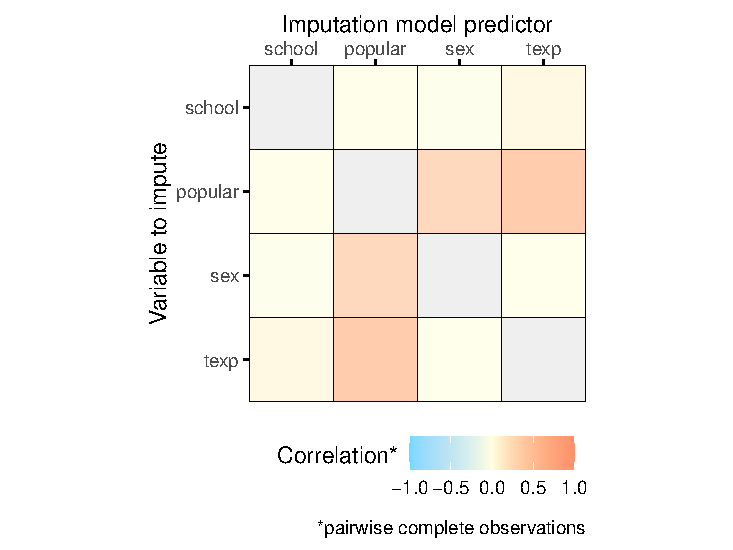
\includegraphics{Imputation_of_Incomplete_Multilevel_Data_files/figure-latex/pop-corr-1} \end{center}

\end{CodeChunk}

This shows us that \texttt{sex} may be a useful imputation model
predictor. Moreover, the missingness in \texttt{popular} may depend on
the observed values of other variables.

\begin{CodeChunk}
\begin{CodeInput}
R> # ggmice(popmis, aes(sex)) +
R> #   geom_histogram(fill = "white") +
R> #   facet_grid(. ~ is.na(popular), scales = "free", labeller = label_both)
R> 
R> ggplot(popmis, aes(y = popular, group = sex)) +
+   geom_boxplot() + 
+   theme_classic()
\end{CodeInput}


\begin{center}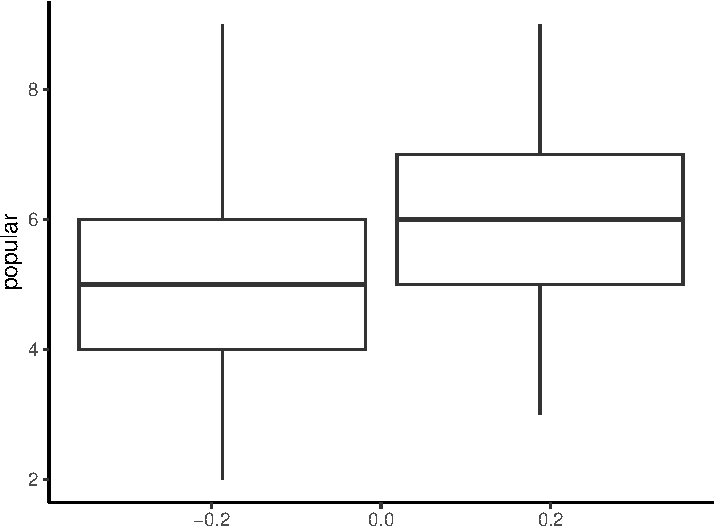
\includegraphics{Imputation_of_Incomplete_Multilevel_Data_files/figure-latex/pop-hist-1} \end{center}

\end{CodeChunk}

\hypertarget{imputation-ignoring-the-cluster-variable-not-recommended}{%
\subsubsection{Imputation ignoring the cluster variable (not
recommended)}\label{imputation-ignoring-the-cluster-variable-not-recommended}}

The first imputation model that we'll use is likely to be invalid. We do
\emph{not} use the cluster identifier \texttt{school} as imputation
model predictor. With this model, we ignore the multilevel structure of
the data, despite the high ICC. This assumes exchangeability between
units. We include it purely to illustrate the effects of ignoring the
clustering in our imputation effort.

Create a methods vector and predictor matrix for \texttt{popular}, and
make sure \texttt{school} is not included as predictor:

\begin{CodeChunk}
\begin{CodeInput}
R> meth <- make.method(popmis) # methods vector
R> pred <- quickpred(popmis)   # predictor matrix
R> plot_pred(pred)
\end{CodeInput}


\begin{center}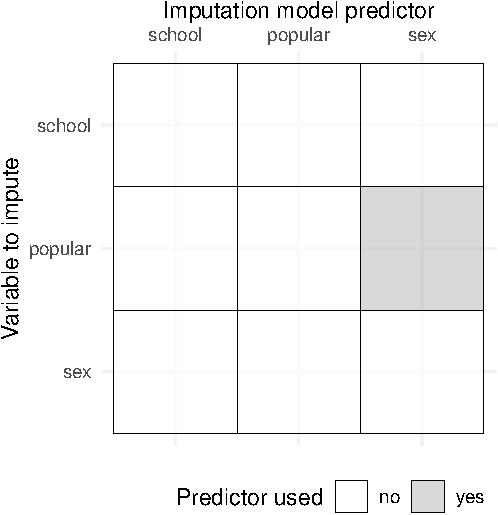
\includegraphics{Imputation_of_Incomplete_Multilevel_Data_files/figure-latex/pop-ignored-pred-1} \end{center}

\end{CodeChunk}

Impute the data, ignoring the cluster structure:

\begin{CodeChunk}
\begin{CodeInput}
R> imp <- mice(popmis, pred = pred, print = FALSE)
\end{CodeInput}
\end{CodeChunk}

Analyze the imputations:

\begin{CodeChunk}
\begin{CodeInput}
R> fit <- with(imp, 
+             lmer(popular ~ 1 + sex  + (1 | school))) 
\end{CodeInput}
\end{CodeChunk}

Print the estimates:

\begin{CodeChunk}
\begin{CodeInput}
R> testEstimates(as.mitml.result(fit), extra.pars = TRUE)
\end{CodeInput}
\begin{CodeOutput}

Call:

testEstimates(model = as.mitml.result(fit), extra.pars = TRUE)

Final parameter estimates and inferences obtained from 5 imputed data sets.

             Estimate Std.Error   t.value        df   P(>|t|)       RIV       FMI 
(Intercept)     5.012     0.295    16.994     4.362     0.000    22.587     0.969 
sex             0.695     0.251     2.768     4.287     0.047    28.390     0.975 

                            Estimate 
Intercept~~Intercept|school    0.266 
Residual~~Residual             1.035 
ICC|school                     0.208 

Unadjusted hypothesis test as appropriate in larger samples.
\end{CodeOutput}
\end{CodeChunk}

\hypertarget{imputation-with-the-cluster-variable-as-predictor-not-recommended}{%
\subsubsection{Imputation with the cluster variable as predictor (not
recommended)}\label{imputation-with-the-cluster-variable-as-predictor-not-recommended}}

We'll now use \texttt{school} as a predictor to impute all other
variables. This is still not recommended practice, since it only works
under certain circumstances and results may be biased
\citep{drec15, ende16}. But at least, it includes some multilevel
aspect. This method is also called `fixed cluster imputation', and uses
N-1 indicator variables representing allocation of N clusters as a fixed
factor in the model \citep{reit06, ende16}. Colloquially, this is
`multilevel imputation for dummies'.

\begin{CodeChunk}
\begin{CodeInput}
R> # adjust the predictor matrix
R> pred["popular", "school"] <- 1 
R> plot_pred(pred)
\end{CodeInput}


\begin{center}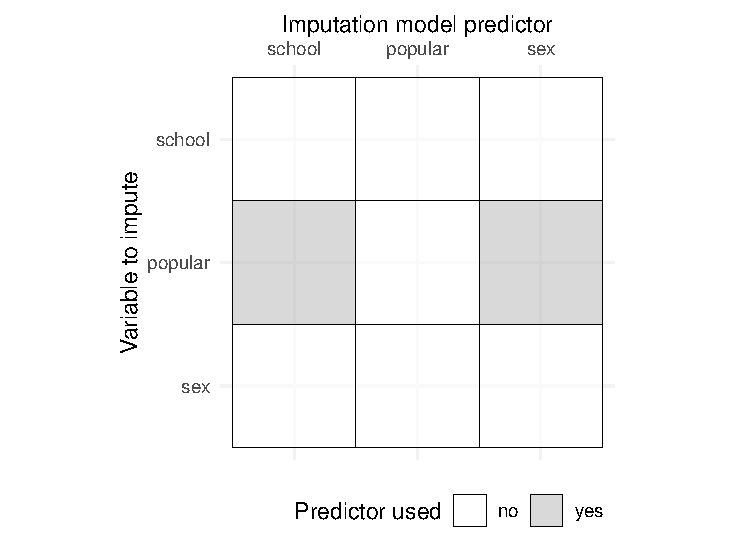
\includegraphics{Imputation_of_Incomplete_Multilevel_Data_files/figure-latex/pop_predictor-1} \end{center}

\begin{CodeInput}
R> # impute the data, cluster as predictor
R> imp <- mice(popmis, pred = pred, print = FALSE)
\end{CodeInput}
\end{CodeChunk}

Analyze the imputations:

\begin{CodeChunk}
\begin{CodeInput}
R> fit <- with(imp, 
+             lmer(popular ~ 1 + sex + (1 | school))) 
\end{CodeInput}
\end{CodeChunk}

Print the estimates:

\begin{CodeChunk}
\begin{CodeInput}
R> testEstimates(as.mitml.result(fit), extra.pars = TRUE)
\end{CodeInput}
\begin{CodeOutput}

Call:

testEstimates(model = as.mitml.result(fit), extra.pars = TRUE)

Final parameter estimates and inferences obtained from 5 imputed data sets.

             Estimate Std.Error   t.value        df   P(>|t|)       RIV       FMI 
(Intercept)     4.915     0.217    22.642     4.926     0.000     9.110     0.926 
sex             0.975     0.283     3.444     4.250     0.024    32.504     0.978 

                            Estimate 
Intercept~~Intercept|school    0.351 
Residual~~Residual             1.153 
ICC|school                     0.233 

Unadjusted hypothesis test as appropriate in larger samples.
\end{CodeOutput}
\end{CodeChunk}

\hypertarget{imputation-with-multilevel-model}{%
\subsubsection{Imputation with multilevel
model}\label{imputation-with-multilevel-model}}

\begin{CodeChunk}
\begin{CodeInput}
R> # adjust the predictor matrix
R> pred["popular", "school"] <- -2 
R> plot_pred(pred)
\end{CodeInput}


\begin{center}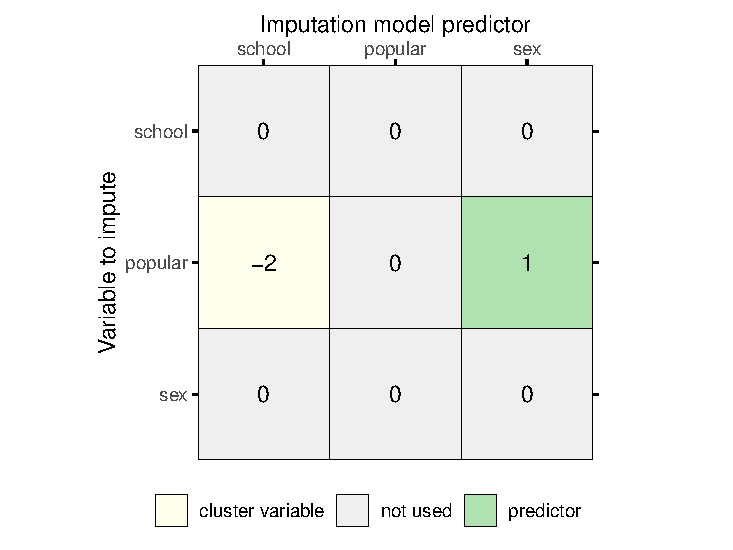
\includegraphics{Imputation_of_Incomplete_Multilevel_Data_files/figure-latex/pop_multilevel-1} \end{center}

\begin{CodeInput}
R> # impute the data, cluster as predictor
R> imp <- mice(popmis, pred = pred, print = FALSE)
\end{CodeInput}
\end{CodeChunk}

Analyze the imputations:

\begin{CodeChunk}
\begin{CodeInput}
R> fit <- with(imp, 
+             lmer(popular ~ 1 + sex + (1 | school))) 
\end{CodeInput}
\end{CodeChunk}

Print the estimates:

\begin{CodeChunk}
\begin{CodeInput}
R> testEstimates(as.mitml.result(fit), extra.pars = TRUE)
\end{CodeInput}
\begin{CodeOutput}

Call:

testEstimates(model = as.mitml.result(fit), extra.pars = TRUE)

Final parameter estimates and inferences obtained from 5 imputed data sets.

             Estimate Std.Error   t.value        df   P(>|t|)       RIV       FMI 
(Intercept)     5.011     0.410    12.222     4.226     0.000    35.955     0.980 
sex             0.928     0.381     2.434     4.168     0.069    48.221     0.985 

                            Estimate 
Intercept~~Intercept|school    0.313 
Residual~~Residual             1.428 
ICC|school                     0.188 

Unadjusted hypothesis test as appropriate in larger samples.
\end{CodeOutput}
\end{CodeChunk}

\hypertarget{case-study-ii-impact-data-syst-missingness-pred-matrix}{%
\section{Case study II: IMPACT data (syst missingness, pred
matrix)}\label{case-study-ii-impact-data-syst-missingness-pred-matrix}}

We illustrate how to impute incomplete multilevel data by means of a
case study: \texttt{impact} from the \pkg{metamisc} package
\citep[empirical data on traumatic brain injuries, \(n = 11,022\) units
across \(N = 15\) clusters,][]{metamisc}. The \texttt{impact} data set
contains traumatic brain injury data on \(n = 11022\) patients clustered
in \(N = 15\) studies with the following 11 variables:

\begin{itemize}
\tightlist
\item
  \texttt{name} Name of the study,
\item
  \texttt{type} Type of study (RCT: randomized controlled trial, OBS:
  observational cohort),
\item
  \texttt{age} Age of the patient,
\item
  \texttt{motor\_score} Glasgow Coma Scale motor score,
\item
  \texttt{pupil} Pupillary reactivity,
\item
  \texttt{ct} Marshall Computerized Tomography classification,
\item
  \texttt{hypox} Hypoxia (0=no, 1=yes),
\item
  \texttt{hypots} Hypotension (0=no, 1=yes),
\item
  \texttt{tsah} Traumatic subarachnoid hemorrhage (0=no, 1=yes),
\item
  \texttt{edh} Epidural hematoma (0=no, 1=yes),
\item
  \texttt{mort} 6-month mortality (0=alive, 1=dead).
\end{itemize}

The analysis model for this dataset is a prediction model with
\texttt{mort} as the outcome. In this tutorial we'll estimate the
adjusted prognostic effect of \texttt{ct} on mortality outcomes. The
estimand is the adjusted odds ratio for \texttt{ct}, after including
\texttt{type}, \texttt{age} \texttt{motor\_score} and \texttt{pupil}
into the analysis model:

\begin{CodeChunk}
\begin{CodeInput}
R> mod <- mort ~ 1 + type + age + motor_score + pupil + ct + (1 | name) 
\end{CodeInput}
\end{CodeChunk}

Note that variables \texttt{hypots}, \texttt{hypox}, \texttt{tsah} and
\texttt{edh} are not part of the analysis model, and may thus serve as
auxiliary variables for imputation.

The \texttt{impact} data included in the \pkg{metamisc} package is a
complete data set. The original data has already been imputed once
(Steyerberg et al, 2008). For the purpose of this tutorial we have
induced missingness (mimicking the missing data in the original data set
before imputation). The resulting incomplete data can be accessed from
\href{https://zenodo.com}{zenodo link to be created}.

Load the complete and incomplete data into the R workspace:

\begin{CodeChunk}
\begin{CodeInput}
R> data("impact", package = "metamisc")      # complete data
R> dat <- read.table("link/to/the/data.txt") # incomplete data
\end{CodeInput}
\end{CodeChunk}

The estimated effects in the complete data are visualized in Figure
\ref{}.

\begin{CodeChunk}


\begin{center}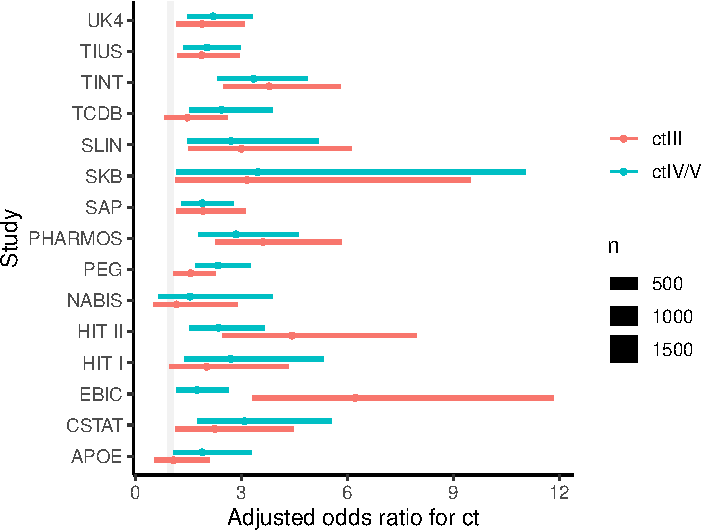
\includegraphics{Imputation_of_Incomplete_Multilevel_Data_files/figure-latex/forest-1} \end{center}

\end{CodeChunk}

\begin{CodeChunk}
\begin{CodeInput}
R> # fit <- glmer(mod, family = "binomial", data = impact) # fit the model
R> # tidy(fit, conf.int = TRUE, exponentiate = TRUE)       # print estimates
\end{CodeInput}
\end{CodeChunk}

\hypertarget{missingness}{%
\subsection{Missingness}\label{missingness}}

To explore the missingness, it is wise to look at the missing data
pattern. The ten most frequent missingness patterns are shown:

\begin{CodeChunk}
\begin{CodeInput}
R> plot_pattern(dat, rotate = TRUE, npat = 10L)  # plot missingness pattern
\end{CodeInput}


\begin{center}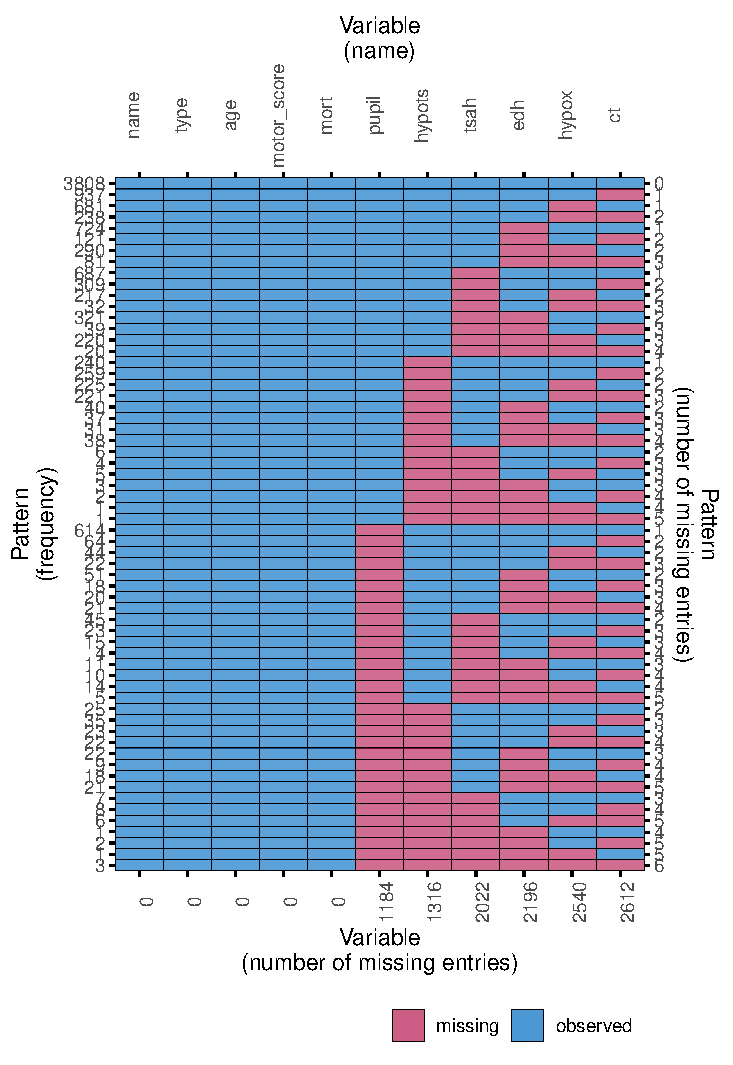
\includegraphics{Imputation_of_Incomplete_Multilevel_Data_files/figure-latex/pattern-1} \end{center}

\end{CodeChunk}

This shows that we need to impute \texttt{ct} and \texttt{pupil}.

To develop the best imputation model, we need to investigate the
relations between the observed values of the incomplete variables and
the observed values of other variables, and the relation between the
missingness indicators of the incomplete variables and the observed
values of the other variables. To see whether the missingness depends on
the observed values of other variables, we can test this statistically
or use visual inspection (e.g.~a histogram faceted by the missingness
indicator).

We should impute the variables \texttt{ct} and \texttt{pupil} and any
auxiliary variables we might want to use to impute these incomplete
analysis model variables. We can evaluate which variables may be useful
auxiliaries by plotting the pairwise complete correlations:

\begin{CodeChunk}
\begin{CodeInput}
R> plot_corr(dat, rotate = TRUE) # plot correlations 
\end{CodeInput}


\begin{center}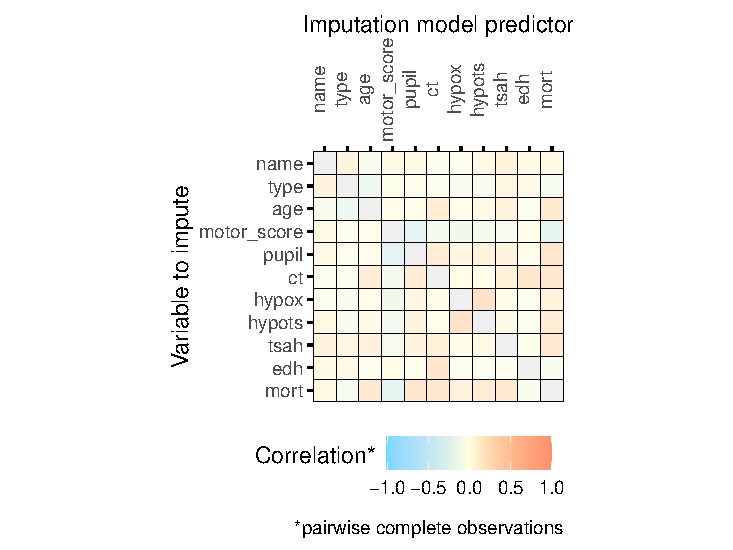
\includegraphics{Imputation_of_Incomplete_Multilevel_Data_files/figure-latex/impact_corr-1} \end{center}

\end{CodeChunk}

This shows us that \texttt{hypox} and \texttt{hypot} would not be useful
auxiliary variables for imputing \texttt{ct}. Depending on the minimum
required correlation, \texttt{tsah} could be useful, while \texttt{edh}
has the strongest correlation with \texttt{ct} out of all the variables
in the data and should definitely be included in the imputation model.
For the imputation of \texttt{pupil}, none of the potential auxiliary
variables has a very strong relation, but \texttt{hypots} could be used.
We conclude that we can exclude \texttt{hypox} from the data, since this
is neither an analysis model variable nor an auxiliary variable for
imputation:

\begin{CodeChunk}
\begin{CodeInput}
R> dat <- select(dat, !hypox)  # remove variable
\end{CodeInput}
\end{CodeChunk}

\hypertarget{complete-case-analysis}{%
\subsection{Complete case analysis}\label{complete-case-analysis}}

As previously stated, complete case analysis lowers statistical power
and may bias results. The complete case analysis estimates are:

\begin{CodeChunk}
\begin{CodeInput}
R> fit <- glmer(mod, family = "binomial", data = na.omit(dat)) # fit the model
R> tidy(fit, conf.int = TRUE, exponentiate = TRUE)             # print estimates
\end{CodeInput}
\begin{CodeOutput}
# A tibble: 11 x 9
   effect   group term        estim~1 std.er~2 stati~3   p.value conf.~4 conf.~5
   <chr>    <chr> <chr>         <dbl>    <dbl>   <dbl>     <dbl>   <dbl>   <dbl>
 1 fixed    <NA>  (Intercept)  0.0863  0.0182   -11.6   2.99e-31  0.0571   0.130
 2 fixed    <NA>  typeRCT      0.757   0.137     -1.54  1.22e- 1  0.531    1.08 
 3 fixed    <NA>  age          1.03    0.00265   12.9   7.40e-38  1.03     1.04 
 4 fixed    <NA>  motor_scor~  0.651   0.0732    -3.82  1.34e- 4  0.522    0.811
 5 fixed    <NA>  motor_scor~  0.489   0.0555    -6.30  2.97e-10  0.391    0.611
 6 fixed    <NA>  motor_scor~  0.274   0.0321   -11.0   2.28e-28  0.218    0.345
 7 fixed    <NA>  pupilNone    3.20    0.317     11.7   8.18e-32  2.63     3.88 
 8 fixed    <NA>  pupilOne     1.75    0.195      5.06  4.27e- 7  1.41     2.18 
 9 fixed    <NA>  ctIII        2.41    0.268      7.89  3.05e-15  1.94     2.99 
10 fixed    <NA>  ctIV/V       2.30    0.214      8.95  3.55e-19  1.92     2.76 
11 ran_pars name  sd__(Inter~  0.230  NA         NA    NA        NA       NA    
# ... with abbreviated variable names 1: estimate, 2: std.error, 3: statistic,
#   4: conf.low, 5: conf.high
\end{CodeOutput}
\end{CodeChunk}

As we can see, a higher \texttt{ct} (Marshall Computerized Tomography
classification) is associated with a lower odds of 6-month mortality,
given by the odds ratio exp(0.42), CI \ldots{} to \ldots, when
controlling for\ldots{}

\hypertarget{imputation-model}{%
\subsection{Imputation model}\label{imputation-model}}

Mutate data to get the right data types for imputation (e.g.~integer for
clustering variable).

\begin{CodeChunk}
\begin{CodeInput}
R> dat <- dat %>% mutate(across(everything(), as.integer))
\end{CodeInput}
\end{CodeChunk}

Create a methods vector and predictor matrix, and make sure
\texttt{name} is not included as predictor, but as clustering variable:

\begin{CodeChunk}
\begin{CodeInput}
R> meth <- make.method(dat) # methods vector
R> pred <- quickpred(dat)   # predictor matrix
R> plot_pred(pred, rotate = TRUE)
\end{CodeInput}


\begin{center}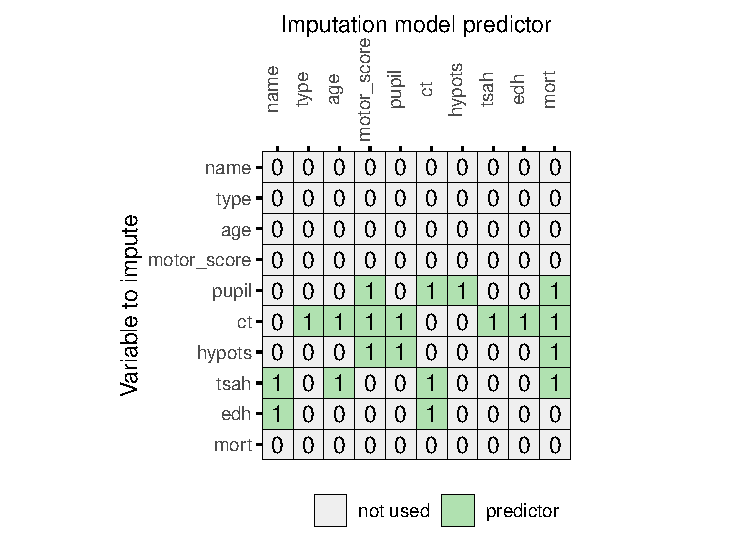
\includegraphics{Imputation_of_Incomplete_Multilevel_Data_files/figure-latex/impact-1} \end{center}

\begin{CodeInput}
R> pred[pred == 1] <- 2
R> pred["mort", ] <- 2
R> pred[, "mort"] <- 2
R> pred[c("name", "type", "age", "motor_score", "mort"), ] <- 0
R> pred[, "name"] <- -2
R> diag(pred) <- 0
R> plot_pred(pred, rotate = TRUE)
\end{CodeInput}


\begin{center}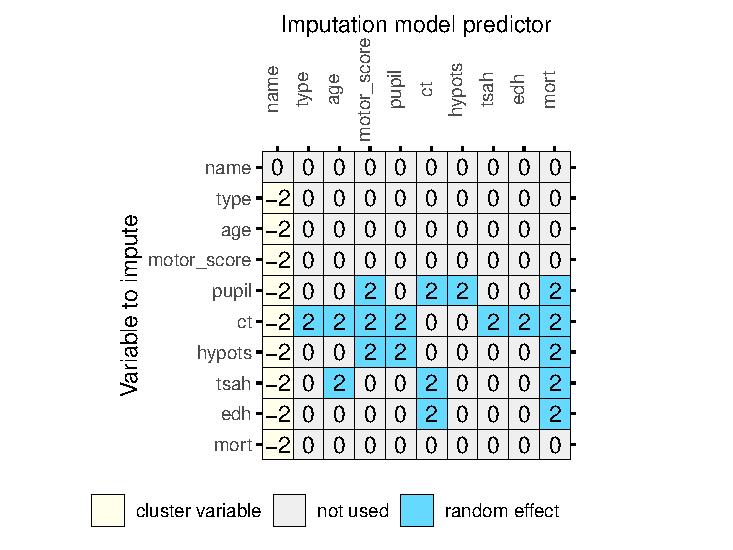
\includegraphics{Imputation_of_Incomplete_Multilevel_Data_files/figure-latex/impact-2} \end{center}

\begin{CodeInput}
R> meth <- make.method(dat)
R> meth
\end{CodeInput}
\begin{CodeOutput}
       name        type         age motor_score       pupil          ct 
         ""          ""          ""          ""       "pmm"       "pmm" 
     hypots        tsah         edh        mort 
      "pmm"       "pmm"       "pmm"          "" 
\end{CodeOutput}
\end{CodeChunk}

Impute the incomplete data

\begin{CodeChunk}
\begin{CodeInput}
R> imp <- mice(dat, method = meth, predictorMatrix = pred, printFlag = FALSE)
\end{CodeInput}
\end{CodeChunk}

\begin{CodeChunk}
\begin{CodeInput}
R> fit <- imp %>% 
+   with(glmer(mort ~ type + age + as.factor(motor_score) + pupil + ct + (1 | name), family = "binomial")) 
R> tidy(pool(fit))
\end{CodeInput}
\begin{CodeOutput}
                     term    estimate   std.error  statistic      p.value
1             (Intercept) -2.35199614 0.340174191  -6.914093 4.993068e-12
2                    type -0.41267936 0.180271952  -2.289204 2.208652e-02
3                     age  0.03049024 0.001570154  19.418637 1.233010e-81
4 as.factor(motor_score)2 -0.66765325 0.068737838  -9.713038 3.478858e-22
5 as.factor(motor_score)3 -1.05520488 0.070218678 -15.027410 2.536132e-50
6 as.factor(motor_score)4 -1.51238928 0.072304221 -20.917026 1.857373e-90
7                   pupil  0.48421506 0.038982924  12.421209 6.781796e-17
8                      ct  0.43474556 0.029968441  14.506779 2.341875e-36
             b          df dfcom         fmi      lambda m         riv
1 5.301620e-04 10113.60453 11013 0.005694385 0.005497777 5 0.005528170
2 4.905995e-05 10892.82806 11013 0.001994781 0.001811557 5 0.001814845
3 3.333628e-08  6323.59900 11013 0.016537098 0.016226102 5 0.016493731
4 4.194026e-05  8322.17049 11013 0.010889419 0.010651742 5 0.010766424
5 5.136864e-05  7631.13821 11013 0.012760548 0.012501842 5 0.012660117
6 1.403437e-04  2830.62134 11013 0.032897234 0.032214161 5 0.033286456
7 3.571667e-04    49.96887 11013 0.309144148 0.282035215 5 0.392825972
8 8.586575e-05   294.70102 11013 0.120676307 0.114728924 5 0.129597506
          ubar
1 1.150823e-01
2 3.243910e-02
3 2.425379e-06
4 4.674562e-03
5 4.869020e-03
6 5.059488e-03
7 1.091068e-03
8 7.950686e-04
\end{CodeOutput}
\begin{CodeInput}
R> as.mitml.result(fit)
\end{CodeInput}
\begin{CodeOutput}
[[1]]
Generalized linear mixed model fit by maximum likelihood (Laplace
  Approximation) [glmerMod]
 Family: binomial  ( logit )
Formula: mort ~ type + age + as.factor(motor_score) + pupil + ct + (1 |  
    name)
      AIC       BIC    logLik  deviance  df.resid 
10495.423 10561.192 -5238.712 10477.423     11013 
Random effects:
 Groups Name        Std.Dev.
 name   (Intercept) 0.2843  
Number of obs: 11022, groups:  name, 15
Fixed Effects:
            (Intercept)                     type                      age  
               -2.37194                 -0.41015                  0.03052  
as.factor(motor_score)2  as.factor(motor_score)3  as.factor(motor_score)4  
               -0.65802                 -1.04611                 -1.51245  
                  pupil                       ct  
                0.50405                  0.42496  
optimizer (Nelder_Mead) convergence code: 0 (OK) ; 0 optimizer warnings; 1 lme4 warnings 

[[2]]
Generalized linear mixed model fit by maximum likelihood (Laplace
  Approximation) [glmerMod]
 Family: binomial  ( logit )
Formula: mort ~ type + age + as.factor(motor_score) + pupil + ct + (1 |  
    name)
     AIC      BIC   logLik deviance df.resid 
10500.88 10566.65 -5241.44 10482.88    11013 
Random effects:
 Groups Name        Std.Dev.
 name   (Intercept) 0.2917  
Number of obs: 11022, groups:  name, 15
Fixed Effects:
            (Intercept)                     type                      age  
               -2.37718                 -0.41511                  0.03067  
as.factor(motor_score)2  as.factor(motor_score)3  as.factor(motor_score)4  
               -0.66935                 -1.05211                 -1.49429  
                  pupil                       ct  
                0.49013                  0.43835  
optimizer (Nelder_Mead) convergence code: 0 (OK) ; 0 optimizer warnings; 1 lme4 warnings 

[[3]]
Generalized linear mixed model fit by maximum likelihood (Laplace
  Approximation) [glmerMod]
 Family: binomial  ( logit )
Formula: mort ~ type + age + as.factor(motor_score) + pupil + ct + (1 |  
    name)
      AIC       BIC    logLik  deviance  df.resid 
10505.026 10570.795 -5243.513 10487.026     11013 
Random effects:
 Groups Name        Std.Dev.
 name   (Intercept) 0.2908  
Number of obs: 11022, groups:  name, 15
Fixed Effects:
            (Intercept)                     type                      age  
               -2.32327                 -0.42365                  0.03023  
as.factor(motor_score)2  as.factor(motor_score)3  as.factor(motor_score)4  
               -0.67143                 -1.05776                 -1.51039  
                  pupil                       ct  
                0.49756                  0.42474  
optimizer (Nelder_Mead) convergence code: 0 (OK) ; 0 optimizer warnings; 1 lme4 warnings 

[[4]]
Generalized linear mixed model fit by maximum likelihood (Laplace
  Approximation) [glmerMod]
 Family: binomial  ( logit )
Formula: mort ~ type + age + as.factor(motor_score) + pupil + ct + (1 |  
    name)
      AIC       BIC    logLik  deviance  df.resid 
10519.511 10585.280 -5250.755 10501.511     11013 
Random effects:
 Groups Name        Std.Dev.
 name   (Intercept) 0.2961  
Number of obs: 11022, groups:  name, 15
Fixed Effects:
            (Intercept)                     type                      age  
               -2.33576                 -0.40872                  0.03039  
as.factor(motor_score)2  as.factor(motor_score)3  as.factor(motor_score)4  
               -0.66477                 -1.05453                 -1.51860  
                  pupil                       ct  
                0.45928                  0.44419  
optimizer (Nelder_Mead) convergence code: 0 (OK) ; 0 optimizer warnings; 1 lme4 warnings 

[[5]]
Generalized linear mixed model fit by maximum likelihood (Laplace
  Approximation) [glmerMod]
 Family: binomial  ( logit )
Formula: mort ~ type + age + as.factor(motor_score) + pupil + ct + (1 |  
    name)
      AIC       BIC    logLik  deviance  df.resid 
10522.038 10587.807 -5252.019 10504.038     11013 
Random effects:
 Groups Name        Std.Dev.
 name   (Intercept) 0.2955  
Number of obs: 11022, groups:  name, 15
Fixed Effects:
            (Intercept)                     type                      age  
               -2.35183                 -0.40576                  0.03064  
as.factor(motor_score)2  as.factor(motor_score)3  as.factor(motor_score)4  
               -0.67469                 -1.06551                 -1.52622  
                  pupil                       ct  
                0.47006                  0.44148  
optimizer (Nelder_Mead) convergence code: 0 (OK) ; 0 optimizer warnings; 1 lme4 warnings 

attr(,"class")
[1] "mitml.result" "list"        
\end{CodeOutput}
\begin{CodeInput}
R> # testEstimates(as.mitml.result(fit))
\end{CodeInput}
\end{CodeChunk}

\hypertarget{case-study-iii-obesity-data}{%
\section{Case study III: obesity
data}\label{case-study-iii-obesity-data}}

Data are simulated and included in the \texttt{miceheckman} package. We
will use the following variables:

\begin{itemize}
\tightlist
\item
  \texttt{region} Cluster variable,
\item
  \texttt{gender} Gender (0=male, 1=female),
\item
  \texttt{age} Age of the patient,
\item
  \texttt{height} Height in meters,
\item
  \texttt{weight} Weight in kilograms,
\item
  `rt`` Response time in minutes (inclusion-restriction variable).
\end{itemize}

The imputation of these data is based on the
\href{https://github.com/johamunoz/Heckman-IPDMA/blob/main/Toy_example.R}{IPDMA
Heckman Github repo}

Load the data:

\begin{CodeChunk}
\begin{CodeInput}
R> data("obesity", package = "miceheckman")
\end{CodeInput}
\end{CodeChunk}

Select relevant variables:

\begin{CodeChunk}
\begin{CodeInput}
R> dat <- select(obesity, -"bmi")
\end{CodeInput}
\end{CodeChunk}

Visualize missing data pattern:

\begin{CodeChunk}
\begin{CodeInput}
R> plot_pattern(dat)
\end{CodeInput}


\begin{center}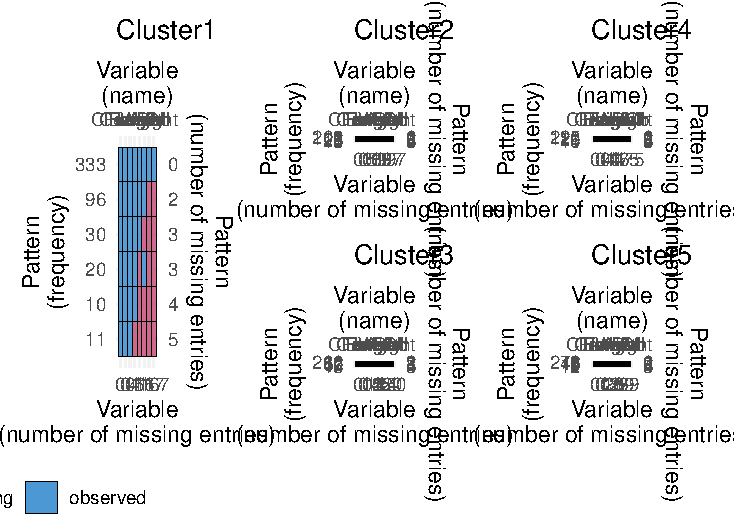
\includegraphics{Imputation_of_Incomplete_Multilevel_Data_files/figure-latex/obesity-md-1} \end{center}

\end{CodeChunk}

Create predictor matrix:

\begin{CodeChunk}
\begin{CodeInput}
R> pred <- quickpred(dat)   # predictor matrix
R> pred["weight","cluster"]<- -2 # clustering variable
R> pred["weight","rt"] <- -3 #inclusion-restriction variable
R> plot_pred(pred)
\end{CodeInput}


\begin{center}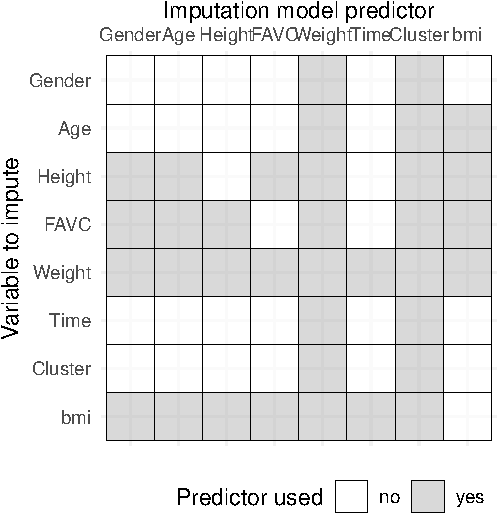
\includegraphics{Imputation_of_Incomplete_Multilevel_Data_files/figure-latex/obesity-pred-1} \end{center}

\end{CodeChunk}

Set the Heckman model as imputation method:

\begin{CodeChunk}
\begin{CodeInput}
R> meth <- make.method(dat) # methods vector
R> meth["weight"]<-"2l.heckman"
\end{CodeInput}
\end{CodeChunk}

Impute the missingness:

\begin{CodeChunk}
\begin{CodeInput}
R> imp <- mice(
+   dat, # dataset with missing values
+   m = 5, # number of imputations
+   maxit = 10,
+   meth = meth, #imputation method vector
+   pred = pred, #imputation predictors matrix
+   meta_method = "reml",
+   printFlag = FALSE
+ )
\end{CodeInput}
\end{CodeChunk}

\hypertarget{discussion}{%
\section{Discussion}\label{discussion}}

\begin{itemize}
\item
  Additional levels of clustering
\item
  More complex data types: timeseries and polynomial relationship in the
  clustering.
\end{itemize}

\hypertarget{funding}{%
\section{Funding}\label{funding}}

This project has received funding from the European Union's Horizon 2020
research and innovation programme under ReCoDID grant agreement No
825746.

The views expressed in this paper are the personal views of the authors
and may not be understood or quoted as being made on behalf of or
reflecting the position of the regulatory agency/agencies or
organizations with which the authors are employed/affiliated.

\hypertarget{references}{%
\section{References}\label{references}}

\bibliography{../References/multilevelmice.bib}



\end{document}
